\documentclass{standalone}
\usepackage{tikz}
\usetikzlibrary{arrows.meta, positioning, shapes.geometric, calc,patterns}

\begin{document}
	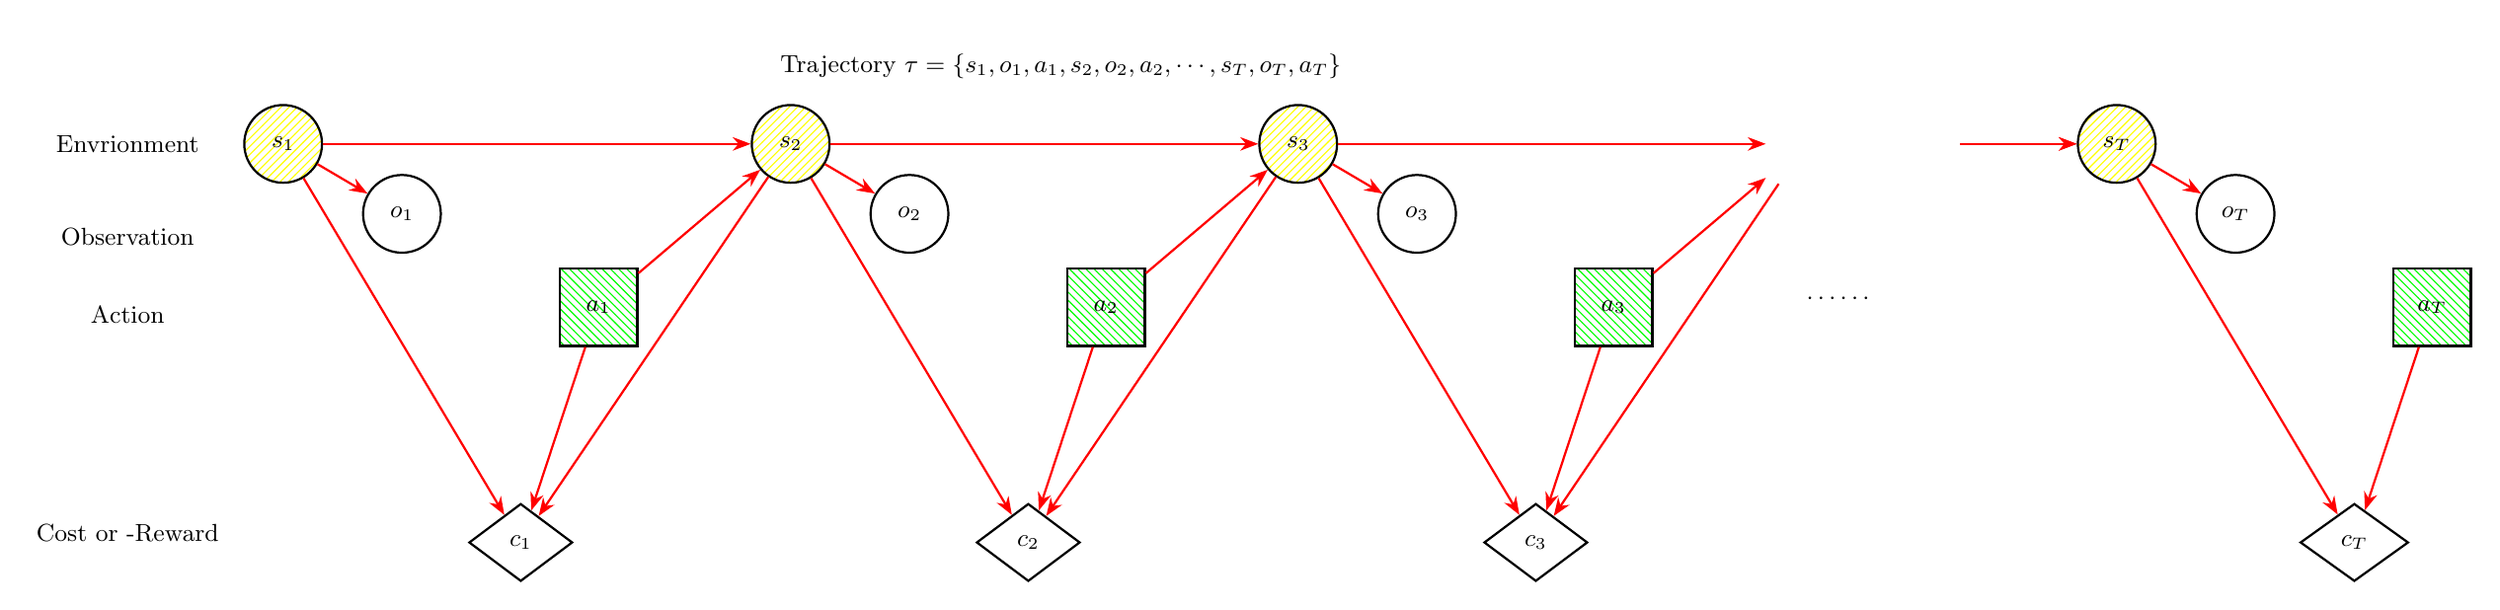
\begin{tikzpicture}[
		node distance=2cm and 1.5cm,
		every node/.style={minimum size=10mm, font=\small},
		cost/.style={draw,diamond, aspect=2, fill=white},
		state/.style={draw,circle,pattern=north east lines, pattern color=yellow},
		obs/.style={draw,circle, fill=white},
		action/.style={draw,rectangle, ,pattern=north west lines, pattern color=green},
		->, >=Stealth, thick, black
		]
		% Diiagram drawing
		\node[state] at (0,0) (s1) {$s_1$};
		\node[obs,right = of s1,xshift = -10mm,yshift = -9mm](o1){$o_1$};
		\node[action,right = of o1,yshift = -12mm](a1){$a_1$};
		\node[cost,below = of a1,xshift = -10mm,yshift = 0mm](c1){$c_1$};
		
		\node [state,right = of s1,xshift = 40mm] (s2) {$s_2$};
		\node[obs,right = of s2,xshift = -10mm,yshift = -9mm](o2){$o_2$};
		\node[action,right = of o2,yshift = -12mm](a2){$a_2$};
		\node[cost,below = of a2,xshift = -10mm,yshift = 0mm](c2){$c_2$};
		
		\node [state,right = of s2,xshift = 40mm] (s3) {$s_3$};
		\node[obs,right = of s3,,xshift = -10mm,yshift = -9mm](o3){$o_3$};
		\node[action,right = of o3,yshift = -12mm](a3){$a_3$};
		\node[cost,below = of a3,xshift = -10mm,yshift = 0mm](c3){$c_3$};		
		

		\node [state,right = of s3,xshift = 80mm] (sT) {$s_T$};
		\node[obs,right = of sT,,xshift = -10mm,yshift = -9mm](oT){$o_T$};
		\node[action,right = of oT,yshift = -12mm](aT){$a_T$};
		\node[cost,below = of aT,xshift = -10mm,yshift = 0mm](cT){$c_T$};	
		
		\node [right = of s3,,xshift = 40mm] (s4) {};
		\node [left = of sT] (sT1) {};
		% Denote 
		\node at (10,1) {Trajectory $\tau = \{s_1,o_1,a_1,s_2,o_2,a_2,\cdots,s_T,o_T,a_T\}$};
		\node at (-2,0) (Envrionment) {Envrionment};
		\node at (-2,-1.2) (Observation){Observation};
		\node at (-2,-2.2)(Action){Action};
		\node at (-2,-5) (Cost){Cost or -Reward};
		\node at (20,-2) {$\cdots \cdots $};
		% draw arrows
		\draw (s1) edge[red] (s2);
		\draw (s2) edge[red] (s3);
		\draw (s3) edge[red] (s4);
		\draw (sT1) edge[red] (sT);
		
		\draw (s1) edge[red] (o1);
		\draw (s2) edge[red] (o2);
		\draw (s3) edge[red] (o3);
		\draw (sT) edge[red] (oT);
		
		\draw (a1) edge[red] (s2);
		\draw (a2) edge[red] (s3);
		\draw (a3) edge[red] (s4);
		\draw (sT1) edge[red] (sT);
		
		\draw (s1) edge[red] (c1);
		\draw (a1) edge[red] (c1);
		\draw (s2) edge[red] (c1);
		
		\draw (s2) edge[red] (c2);
		\draw (a2) edge[red] (c2);
		\draw (s3) edge[red] (c2);
		
		\draw (s3) edge[red] (c3);
		\draw (a3) edge[red] (c3);
		\draw (s4) edge[red] (c3);
		
		\draw (sT) edge[red] (cT);
		\draw (aT) edge[red] (cT);	
%		\node[cost] at (-7,0) (costnode) {$c$};
%		\node[draw = white,right= of costnode,xshift = -10mm,align=center]  {Cost or Loss \\ or negative Utility \\or negative Reward};
%		\node[shaded, below = of costnode, yshift = 17mm] (statenode) {$s$};
%		\node[draw = white, right = of statenode,xshift = -10mm,align = center] {State Random Variable};
%		\node[obs, below= of statenode,yshift = 17mm]  (obsnode) {$o$};
%		\node[draw = white, right = of obsnode,xshift = -10mm,align = center]  {Output from SHM result};
%		\node[action,below = of obsnode,yshift = 17mm]  (actionnode) {$a$};
%		\node[draw = white, right = of actionnode,xshift = -10mm, align=center] {Action or Decision };
		
	\end{tikzpicture}
\end{document}
